\documentclass[tikz]{standalone}
\usepackage{amsmath,amssymb}
\usepackage{tikz}
\usetikzlibrary{
	shapes,
	snakes,
	calc,
	decorations,
	decorations.markings,
	decorations.text,
	decorations.pathreplacing}
	
\begin{document}
\begin{tikzpicture}[scale=1,auto,every text node part/.style={align=center}]
  \definecolor{darkred}{rgb}{0.75,0,0}
  \definecolor{darkblue}{rgb}{0,0,0.75}
  \definecolor{darkgreen}{rgb}{0,0.75,0}

  
%%   \node[darkgreen] (More) at (0,0) {
%%     \begin{tikzpicture}
%%       \node (M0) at (0,2.4) {More(one hundred one, fifty two)\\
%%         \tiny$\text{More}(P B S,Q C T) \leftarrow \text{LargerBase}(B,C), \text{Prefix}(P,B), \text{Suffix}(B,S), \text{Prefix}(Q,C), \text{Suffix}(C,T).$};
%%       
%%       \node (LB1) at (-10,1.2) {LargerBase(hundred, $\varnothing$).\\
%%         \tiny$\text{LargerBase}(X,Y) \leftarrow \text{PrevBase}(X,Y).$};
%%       \node (P2) at (-11,0) {Prefix($\varnothing$, $\varnothing$).};
%%       
%%       \node (P1) at (-5,1.2) {Prefix(one, hundred)\\
%%         \tiny$\text{Prefix}(P,hundred) \leftarrow \text{Ones}(P).$};
%%       \node (O2) at (-6.5,0) {Ones(one).};
%%       
%%       \node (S1) at (0,1.2) {Suffix(hundred, one)\\
%%         \tiny$\text{Suffix}(B,PCS) \leftarrow \text{LargerBase}(B,C), \text{Number}(PCS).$};
%%       \node (LB2) at (-3,0) {LargerBase(hundred, $\varnothing$).\\
%%         \tiny$\text{LargerBase}(X,Y) \leftarrow \text{PrevBase}(X,Y).$};
%%       \node (P3) at (-3,-1.2) {Prefix($\varnothing$, $\varnothing$).};
%%       \node (N2) at (1.5,0) {Number(one)\\
%%         \tiny$\text{Number}(PBS) \leftarrow \text{Prefix}(P,C), \text{Suffix}(C,S).$};
%%       \node (Pr3) at (-.5,-1.2) {Prefix($\varnothing$, $\varnothing$).};
%%       \node (Su3) at (3,-1.2) {Suffix($\varnothing$, one)\\
%%         \tiny$\text{Suffix}(\varnothing, X) \leftarrow \text{Ones}(Y).$};
%%       \node (O4) at (1.5,-2.4) {Ones(one).};
%%       
%%       \node (Pr1) at (5,1.2) {Prefix($\varnothing$, $\varnothing$).};
%% 
%%       \node (Su1) at (9,1.2) {Suffix($\varnothing$, fifty two)\\
%%         \tiny$\text{Suffix}(\varnothing,XY) \leftarrow \text{Decades}(X), \text{Ones}(Y).$};
%%       \node (D2) at (7.5,0) {Decades(fifty).};
%%       \node (On2) at (10,0) {Ones(two).};
%%             
%%       \draw [<-] (M0)     to (LB1);
%%       \draw [<-] (M0)     to (P1);
%%       \draw [<-] (M0)     to (S1);
%%       \draw [<-] (M0)     to (Pr1);
%%       \draw [<-] (M0)     to (Su1);
%%       \draw [<-] (LB1)    to (P2);
%%       \draw [<-] (P1)     to (O2);
%%       \draw [<-] (S1)     to (LB2);
%%       \draw [<-] (S1)     to (N2);
%%       \draw [<-] (LB2)     to (P3);
%%       \draw [<-] (N2)     to (Pr3);
%%       \draw [<-] (N2)     to (Su3);
%%       \draw [<-] (Su3)     to (O4);
%%       \draw [<-] (Su1)     to (D2);
%%       \draw [<-] (Su1)    to (On2);
%%   \end{tikzpicture}};

  \node[darkgreen] (More) at (2,0) {
    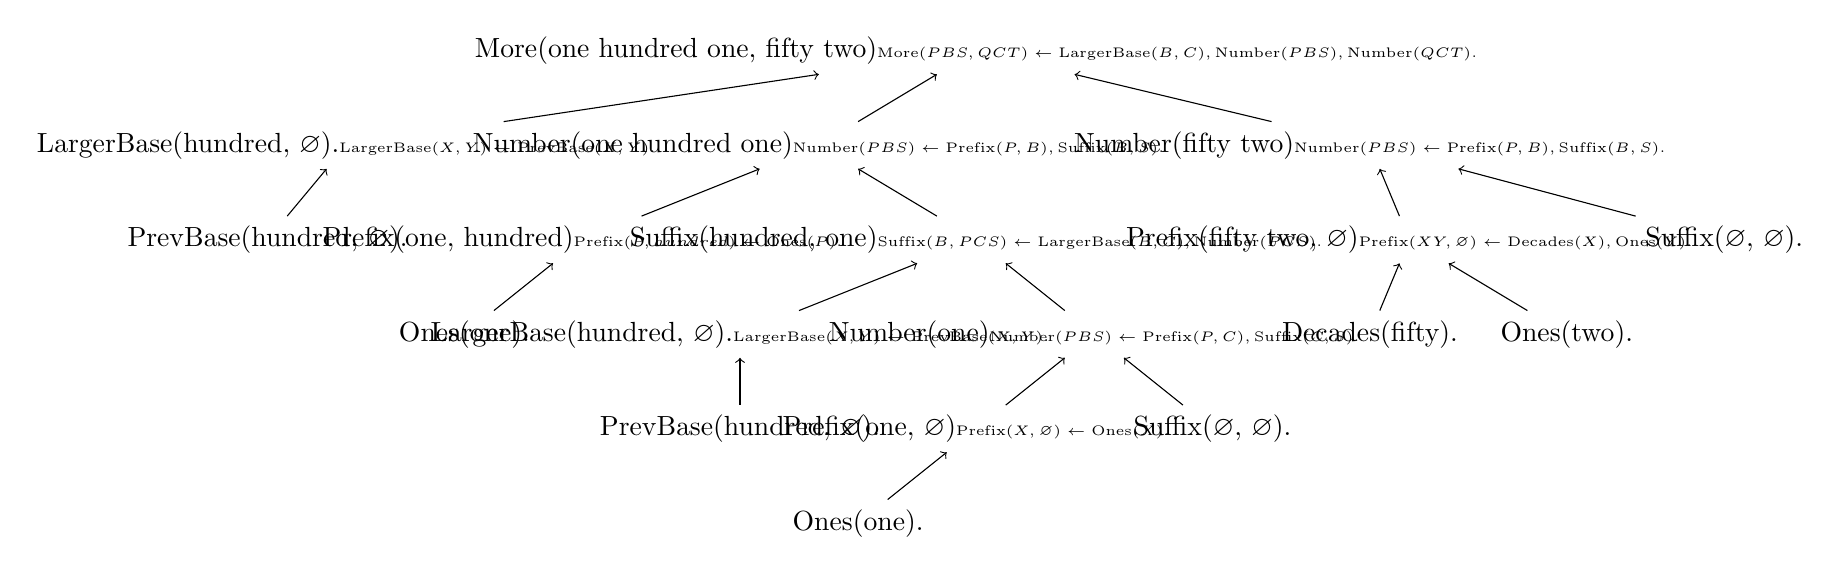
\begin{tikzpicture}
      \node (M0) at (0,3.6) {More(one hundred one, fifty two)\\
        \tiny$\text{More}(P B S,Q C T) \leftarrow \text{LargerBase}(B,C), \text{Number}(PBS), \text{Number}(QCT).$};
      
      \node (LB1) at (-8,2.4) {LargerBase(hundred, $\varnothing$).\\
        \tiny$\text{LargerBase}(X,Y) \leftarrow \text{PrevBase}(X,Y).$};
      \node (P2) at (-9,1.2) {PrevBase(hundred, $\varnothing$).\\};

      \node (N1) at (-2,2.4) {Number(one hundred one)\\
        \tiny$\text{Number}(PBS) \leftarrow \text{Prefix}(P,B), \text{Suffix}(B,S).$};
    
      \node (Nu1) at (5,2.4) {Number(fifty two)\\
        \tiny$\text{Number}(PBS) \leftarrow \text{Prefix}(P,B), \text{Suffix}(B,S).$};
  
      \node (P1) at (-5,1.2) {Prefix(one, hundred)\\
        \tiny$\text{Prefix}(P,hundred) \leftarrow \text{Ones}(P).$};
      \node (O2) at (-6.5,0) {Ones(one).\\};
      
      \node (S1) at (0,1.2) {Suffix(hundred, one)\\
        \tiny$\text{Suffix}(B,PCS) \leftarrow \text{LargerBase}(B,C), \text{Number}(PCS).$};
      \node (LB2) at (-3,0) {LargerBase(hundred, $\varnothing$).\\
        \tiny$\text{LargerBase}(X,Y) \leftarrow \text{PrevBase}(X,Y).$};
      \node (P3) at (-3,-1.2) {PrevBase(hundred, $\varnothing$).\\};
      \node (N2) at (1.5,0) {Number(one)\\
        \tiny$\text{Number}(PBS) \leftarrow \text{Prefix}(P,C), \text{Suffix}(C,S).$};
      \node (Pr3) at (3,-1.2) {Suffix($\varnothing$, $\varnothing$).\\};
      \node (Su3) at (0,-1.2) {Prefix(one, $\varnothing$)\\
        \tiny$\text{Prefix}(X, \varnothing) \leftarrow \text{Ones}(X).$};
      \node (O4) at (-1.5,-2.4) {Ones(one).};
      
      \node (Pr1) at (9.5,1.2) {Suffix($\varnothing$, $\varnothing$).\\};

      \node (Su1) at (5.5,1.2) {Prefix(fifty two, $\varnothing$)\\
        \tiny$\text{Prefix}(X Y, \varnothing) \leftarrow \text{Decades}(X), \text{Ones}(Y).$};
      \node (D2) at (5,0) {Decades(fifty).\\};
      \node (On2) at (7.5,0) {Ones(two).\\};
            
      \draw [<-] (M0)     to (LB1);
      \draw [<-] (M0)     to (N1);
      \draw [<-] (M0)     to (Nu1);
      \draw [<-] (N1)     to (P1);
      \draw [<-] (N1)     to (S1);
      \draw [<-] (Nu1)     to (Pr1);
      \draw [<-] (Nu1)     to (Su1);
      \draw [<-] (LB1)    to (P2);
      \draw [<-] (P1)     to (O2);
      \draw [<-] (S1)     to (LB2);
      \draw [<-] (S1)     to (N2);
      \draw [<-] (LB2)     to (P3);
      \draw [<-] (N2)     to (Pr3);
      \draw [<-] (N2)     to (Su3);
      \draw [<-] (Su3)     to (O4);
      \draw [<-] (Su1)     to (D2);
      \draw [<-] (Su1)    to (On2);
  \end{tikzpicture}};

  \node[anchor=north,darkblue] (Number) at (-5.5,-1.2) {
  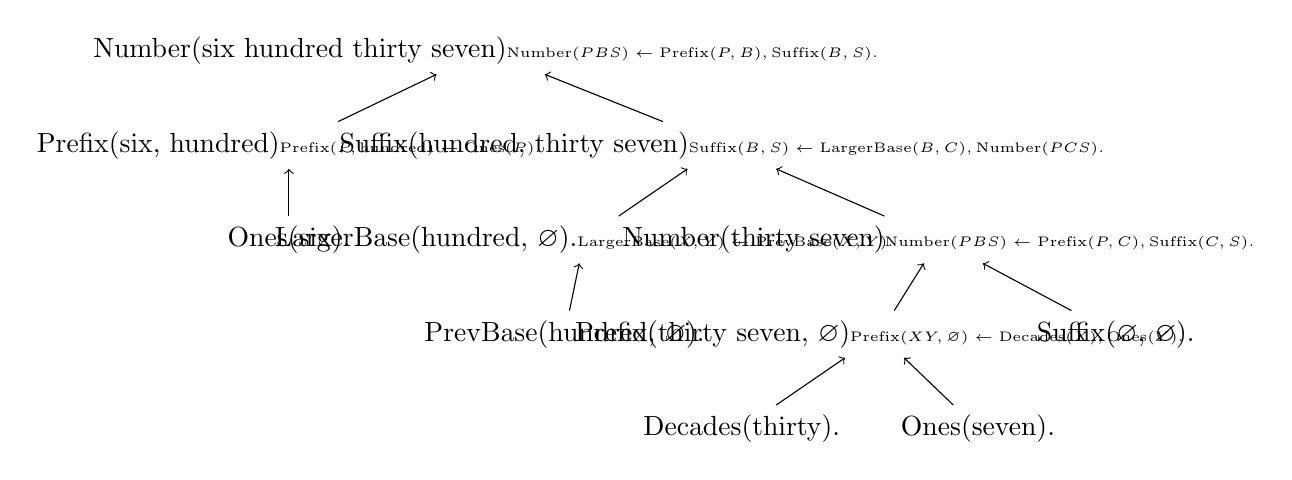
\begin{tikzpicture}
    \node (N0) at (0,2.4) {Number(six hundred thirty seven)\\
      \tiny$\text{Number}(PBS) \leftarrow \text{Prefix}(P,B), \text{Suffix}(B,S).$};
    \node (P1) at (-2.5,1.2) {Prefix(six, hundred)\\
      \tiny$\text{Prefix}(P,\text{hundred}) \leftarrow \text{Ones}(P).$};
    \node (S1) at (3,1.2) {Suffix(hundred, thirty seven)\\
      \tiny$\text{Suffix}(B,S) \leftarrow \text{LargerBase}(B,C), \text{Number}(PCS).$};
    \node (O2) at (-2.5,0) {Ones(six).\\};
    \node (LB2) at (1.25,0) {LargerBase(hundred, $\varnothing$).\\
      \tiny$\text{LargerBase}(X,Y) \leftarrow \text{PrevBase}(X,Y).$};
    \node (N2) at (5.75,0) {Number(thirty seven)\\
      \tiny$\text{Number}(PBS) \leftarrow \text{Prefix}(P,C), \text{Suffix}(C,S).$};
    \node (P3) at (8,-1.2) {Suffix($\varnothing$, $\varnothing$).};
    \node (S3) at (5,-1.2) {Prefix(thirty seven, $\varnothing$)\\
      \tiny$\text{Prefix}(X Y,\varnothing) \leftarrow \text{Decades}(X), \text{Ones}(Y).$};
    \node (D3) at (3.25,-2.4) {Decades(thirty).};
    \node (O3) at (6.25,-2.4) {Ones(seven).};
    \node (PB3) at (1,-1.2) {PrevBase(hundred, $\varnothing$).};

    
    \draw [<-] (N0) to (P1);
    \draw [<-] (N0) to (S1);
    \draw [<-] (P1) to (O2);
    \draw [<-] (S1) to (LB2);
    \draw [<-] (LB2) to (PB3);
    \draw [<-] (S1) to (N2);
    \draw [<-] (N2) to (P3);
    \draw [<-] (N2) to (S3);
    \draw [<-] (S3) to (D3);
    \draw [<-] (S3) to (O3);
  \end{tikzpicture}};
  


  \node[anchor=north,darkred] (Succ) at (9,-2.4) {
    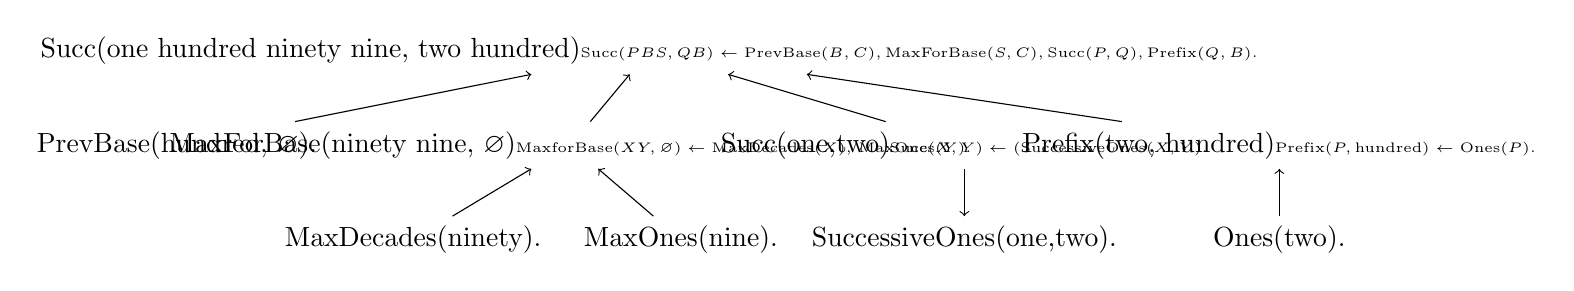
\begin{tikzpicture}
      \node (S0) at (0,2.4) {Succ(one hundred ninety nine, two hundred)\\
        \tiny$\text{Succ}(PBS,QB) \leftarrow \text{PrevBase}(B,C), \text{MaxForBase}(S,C), \text{Succ}(P,Q), \text{Prefix}(Q,B).$};
      
      \node (PB1) at (-6,1.2) {PrevBase(hundred, $\varnothing$).\\};

      \node (MFB1) at (-1,1.2) {MaxForBase(ninety nine, $\varnothing$)\\
        \tiny$\text{MaxforBase}(XY,\varnothing) \leftarrow \text{MaxDecades}(X),\,\text{MaxOnes}(Y).$};
      \node (MD2) at (-3,0) {MaxDecades(ninety).};
      \node (MO2) at (0.4,0) {MaxOnes(nine).};

      \node (S1) at (4,1.2) {Succ(one,two)\\
        \tiny$\text{Succ}(X,Y) \leftarrow (\text{SuccessiveOnes}(X,Y).$\\};
      \node (SO2) at (4,0) {SuccessiveOnes(one,two).\\};

      \node (P1) at (8,1.2) {Prefix(two, hundred)\\
        \tiny$\text{Prefix}(P,\text{hundred}) \leftarrow \text{Ones}(P).$};
      \node (O2) at (8,0) {Ones(two).\\};
      
      \draw [<-] (S0)     to (MFB1);
      \draw [<-] (S0)     to (PB1);
      \draw [<-] (S0)     to (P1);
      \draw [<-] (S0)     to (S1);
      \draw [<-] (MFB1)   to (MD2);
      \draw [<-] (MFB1)   to (MO2);
      \draw [<-] (SO2)     to (S1);
      \draw [<-] (P1)     to (O2);
  \end{tikzpicture}};
  
%%   \node[anchor=north,darkred] (Succ) at (6.5,-2.4) {
%%     \begin{tikzpicture}
%%       \node (S0) at (0,2.4) {Succ(ninety nine, one hundred)\\
%%         \tiny$\text{Succ}(X,\text{one}\,C) \leftarrow \text{MaxForBase}(X,B), \text{PrevBase}(C,B).$};
%%       \node (MFB1) at (-3,1.2) {MaxForBase(ninety nine, $\varnothing$)\\
%%         \tiny$\text{MaxforBase}(XY,\varnothing) \leftarrow \text{MaxDecades}(X),\,\text{MaxOnes}(Y).$};
%%       \node (PB1) at (2.5,1.2) {PrevBase(hundred, $\varnothing$).\\};
%%       \node (MD2) at (-4,0) {MaxDecades(ninety).};
%%       \node (MO2) at (-.5,0) {MaxOnes(nine).};
%%       
%%       \draw [<-] (S0)     to (MFB1);
%%       \draw [<-] (S0)     to (PB1);
%%       \draw [<-] (MFB1)  to (MD2);
%%       \draw [<-] (MFB1)  to (MO2);
%%     \end{tikzpicture}};
\end{tikzpicture}
\end{document}
